\documentclass[tikz,border=3pt]{standalone}
\usepackage{amsmath}
\usepackage{helvet}
\renewcommand{\familydefault}{\sfdefault}
\usetikzlibrary{arrows.meta,positioning,fit,calc}
\definecolor{mobo}{RGB}{224,239,249}
\definecolor{llm}{RGB}{255,238,205}
\definecolor{sim}{RGB}{232,242,228}
\definecolor{state}{RGB}{238,238,238}
\definecolor{edge}{RGB}{70,70,70}
\tikzset{
 box/.style={draw=edge, rounded corners=1.5pt, line width=.65pt, align=center,
             inner xsep=5pt, inner ysep=4pt, font=\fontsize{8.2}{9.2}\selectfont},
 flow/.style={-{Latex[length=2.2mm,width=1.4mm]}, line width=.65pt, draw=edge},
 small/.style={font=\fontsize{7.2}{8.0}\selectfont, align=center},
 group/.style={draw=edge!60, rounded corners=2pt, dashed, inner sep=5pt}
}
\begin{document}
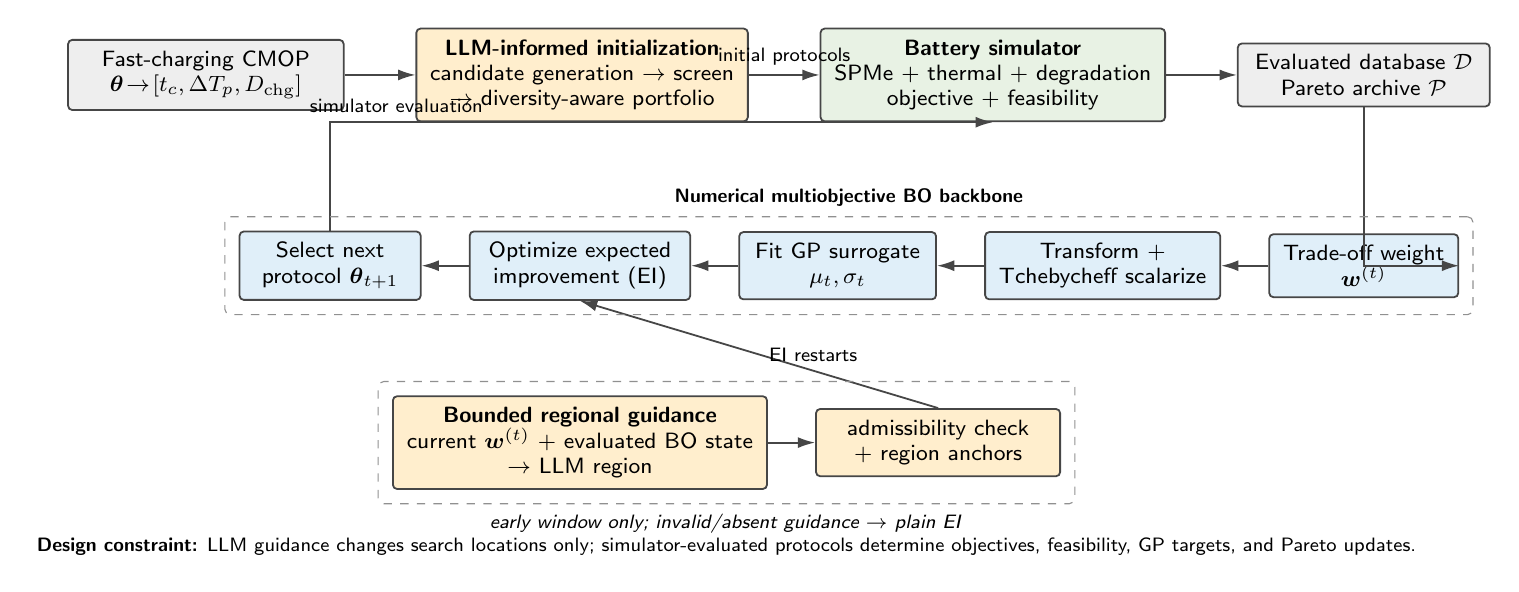
\begin{tikzpicture}[node distance=5mm and 6.5mm]

\node[box, fill=state, minimum width=35mm] (problem) {Fast-charging CMOP\\$\boldsymbol\theta\!\rightarrow\![t_c,\Delta T_p,D_{\rm chg}]$};
\node[box, fill=llm, minimum width=39mm, right=9mm of problem] (init) {\textbf{LLM-informed initialization}\\candidate generation $\rightarrow$ screen\\$\rightarrow$ diversity-aware portfolio};
\node[box, fill=sim, minimum width=32mm, right=9mm of init] (simulator) {\textbf{Battery simulator}\\SPMe + thermal + degradation\\objective + feasibility};
\node[box, fill=state, minimum width=32mm, right=9mm of simulator] (database) {Evaluated database $\mathcal D$\\Pareto archive $\mathcal P$};

\draw[flow] (problem) -- (init);
\draw[flow] (init) -- node[small,above]{initial protocols} (simulator);
\draw[flow] (simulator) -- (database);

\node[box, fill=mobo, minimum width=24mm, below=16mm of database] (weight) {Trade-off weight\\$\boldsymbol w^{(t)}$};
\node[box, fill=mobo, minimum width=29mm, left=6mm of weight] (scalar) {Transform +\\Tchebycheff scalarize};
\node[box, fill=mobo, minimum width=25mm, left=6mm of scalar] (gp) {Fit GP surrogate\\$\mu_t,\sigma_t$};
\node[box, fill=mobo, minimum width=28mm, left=6mm of gp] (ei) {Optimize expected\\improvement (EI)};
\node[box, fill=mobo, minimum width=23mm, left=6mm of ei] (candidate) {Select next\\protocol $\boldsymbol\theta_{t+1}$};

\draw[flow] (database.south) |- (weight.east);
\draw[flow] (weight) -- (scalar);
\draw[flow] (scalar) -- (gp);
\draw[flow] (gp) -- (ei);
\draw[flow] (ei) -- (candidate);
\draw[flow] (candidate.north) |- node[small,pos=.55,above]{simulator evaluation} (simulator.south);

\node[box, fill=llm, minimum width=34mm, below=12mm of ei] (region) {\textbf{Bounded regional guidance}\\current $\boldsymbol w^{(t)}$ + evaluated BO state\\$\rightarrow$ LLM region};
\node[box, fill=llm, minimum width=31mm, right=6mm of region] (anchors) {admissibility check\\+ region anchors};
\draw[flow] (region) -- (anchors);
\draw[flow] (anchors.north) -- node[small,right]{EI restarts} (ei.south);

\node[group, fit=(weight)(scalar)(gp)(ei)(candidate), label={[small]above:\textbf{Numerical multiobjective BO backbone}}] (mgroup) {};
\node[group, fit=(region)(anchors), label={[small]below:\textit{early window only; invalid/absent guidance $\rightarrow$ plain EI}}] (rgroup) {};

\node[small, below=3mm of rgroup] (note) {\textbf{Design constraint:} LLM guidance changes search locations only; simulator-evaluated protocols determine objectives, feasibility, GP targets, and Pareto updates.};

\end{tikzpicture}
\end{document}
